\documentclass[11pt,a4paper]{article}

\usepackage[utf8]{inputenc}		% Configuro la codificación
\input{.command.tex}
% En el siguiente archivo se configuran las variables del trabajo práctico
%% \providecommand es similar a \newcommnad, salvo que el primero ante un 
%% conflicto en la compilación, es ignorado.

% Al comienzo de un TP se debe modificar los argumentos de los comandos


\providecommand{\myTitle}{TRABAJO PRÁCTICO ESPECIAL}
\providecommand{\mySubtitle}{Análisis y procesamiento de la señal de habla}

\providecommand{\mySubject}{Señales y Sistemas (85.05)}
\providecommand{\myKeywords}{UBA, Ingeniería, 85.05, Señales y Sistemas}

% No es necesario modificar este
\providecommand{\myHeaderLogo}{header_fiuba}

\providecommand{\myAuthorSurname}{Manso}
\providecommand{\myTimePeriod}{Año 2016 - 2\textsuperscript{do} Cuatrimestre}


% Crear los integrantes del TP con el comando \PutMember donde
%%		1) Apellido, Nombre
%%		2) Número de Padrón
%%		3) E-Mail (Si el mail contiene '_', escribirlos como '\_'
\providecommand{\CoverMembers}[0]{
		\PutMember{Manso, Juan} {96133} {juanmanso@gmail.com}
}

\providecommand{\myLstLanguage}{Octave}

\Pagebreakfalse		% Setea si hay un salto de página en la carátula
\Indexfalse
\Siunitxfalse		% Si quiero utilizar el paquete, \siunixtrue. Si no \siunitxfalse
\Listingstrue		% Idem con paquete listings (programación)
\Keywordsfalse
				% Archivo con los comandos globales como Título y autores
%Preambulo para articulo científico de LaTeX

\usepackage[a4paper,left=3cm,right=3cm,bottom=3.5cm,top=3.5cm]{geometry} 	% Configuro la geometría del papel
%\usepackage{microtype}														% Mejora el "spacing" de las palabras
\usepackage[spanish]{babel} 												% Compatibilizo los signos del español
	\addto\captionsspanish{\renewcommand{\tablename}{Tabla}}				%% Redefino nombres preestablecidos por Babel
	\addto\captionsspanish{\renewcommand{\listtablename}{Índice de tablas}}	%% y así en vez de Cuadro dirá Tabla.
\usepackage{amsmath, amsfonts, amssymb}										% Entornos matemáticos, fuentes y símbolos
\usepackage{graphicx}														% Necesario para insertar figuras
\usepackage{fancyhdr}														% Para manipular headers y footers
\usepackage[usenames]{color}											% \color{color deseado} {lo que querés que tenga color}
\usepackage{subcaption}														% Permite captions del tipo 1a, 1b
\usepackage{multirow}														% Para tablas
\usepackage{float}

\ifListings
	\usepackage{listingsutf8}

	\definecolor{mygreen}{rgb}{0,0.6,0}
	\definecolor{mygray}{rgb}{0.5,0.5,0.5}
	\definecolor{mymauve}{rgb}{0.58,0,0.82}
	
	\providecommand{\lstinputpath}[1]{\lstset{inputpath=#1}}

	\lstset{
		backgroundcolor=\color{white},   % choose the background color; you must add \usepackage{color} or \usepackage{xcolor}
		inputencoding=utf8/latin1,
		basicstyle=\ttfamily\footnotesize,        % the size of the fonts that are used for the code
		breakatwhitespace=false,         % sets if automatic breaks should only happen at whitespace
		breaklines=true,                 %% sets automatic line breaking
		captionpos=t,                    %% sets the caption-position to top 
		commentstyle=\color{mygreen},    % comment style
		deletekeywords={...},            % if you want to delete keywords from the given language
		escapeinside={\%*}{*)},          % if you want to add LaTeX within your code
		extendedchars=true,              % lets you use non-ASCII characters; for 8-bits encodings only, does not work with UTF-8
		frame=single,	                 %% adds a frame around the code
		keepspaces=true,                 % keeps spaces in text, useful for keeping indentation of code (possibly needs columns=flexible)
		keywordstyle=\color{blue},       % keyword style
		language=C++,		 	 %% the language of the code
		otherkeywords={*,...},           % if you want to add more keywords to the set
		numbers=left,                    %% where to put the line-numbers; possible values are (none, left, right)
		numbersep=5pt,                   %% how far the line-numbers are from the code
		numberstyle=\tiny\color{mygray}, % the style that is used for the line-numbers
		rulecolor=\color{black},         % if not set, the frame-color may be changed on line-breaks within not-black text (e.g. comments (green here))
		showspaces=false,                % show spaces everywhere adding particular underscores; it overrides 'showstringspaces'
		showstringspaces=false,          % underline spaces within strings only
		showtabs=false,                  % show tabs within strings adding particular underscores
		stepnumber=1,                    % the step between two line-numbers. If it's 1, each line will be numbered
		stringstyle=\color{mymauve},     % string literal style
		tabsize=4,	                   % sets default tabsize to 2 space
		title={\protect\filename@parse{\lstname}\protect\filename@base\text{.}\protect\filename@ext}	 %% show the filename of files included with \lstinputlisting; also try caption instead of title
	}
	 \usepackage{algpseudocode}						% Para pseudocodigo
	 \renewcommand{\algorithmicwhile}{\textbf{mientras}} 
	 \renewcommand{\algorithmicdo}{\textbf{hacer}} 
	 \renewcommand{\algorithmicfor}{\textbf{para}}
	 \renewcommand{\algorithmicreturn}{\textbf{devolver}}
	 \renewcommand{\algorithmicend}{\textbf{fin}} 
	 
	 \newcommand{\rpm}{\raisebox{.2ex}{$\scriptstyle\pm$}}  
\fi

\ifSiunitx
\usepackage{siunitx}											% Unidades: \SI {cantidad} {\unidad} (necesita texlive-science)
	\sisetup{load-configurations = abbreviations}							% Habilita poner \cm en vez de \centi\metre
	\sisetup{output-decimal-marker = {,}}									% Cambia los puntos decimales por comas
\fi

\usepackage{booktabs}														% Permite hacer tablas sin separadores en el medio
\usepackage{placeins}														
		\let\Oldsection\section												%% Permite que los flotantes (como figuras) no aparescan
	\renewcommand{\section}{\FloatBarrier\Oldsection}						%% antes o después de su sección correspondiente.
		\let\Oldsubsection\subsection
	\renewcommand{\subsection}{\FloatBarrier\Oldsubsection}		
		\let\Oldsubsubsection\subsubsection
	\renewcommand{\subsubsection}{\FloatBarrier\Oldsubsubsection}
\usepackage{hyperref}														% Debe ser agregado al final del preambulo

\hypersetup
{    bookmarks=true,         % show bookmarks bar?
     unicode=false,          % non-Latin characters in Acrobat’s bookmarks
     pdftoolbar=true,        % show Acrobat’s toolbar?
     pdfmenubar=true,        % show Acrobat’s menu?
     pdffitwindow=false,     % window fit to page when opened
     pdftitle={\myTitle},    		 % title
     pdfauthor={\myAuthorSurname},   % author
	 pdfcreator={\myAuthorSurname},	 % creator = author
     pdfsubject={\mySubject},		 % subject of the document
     pdfkeywords={\myKeywords},
     colorlinks=true,        % false: boxed links; true: colored links
     linkcolor=black,        % color of internal links (change box color with linkbordercolor)
     citecolor=black,        % color of links to bibliography
     filecolor=magenta,      % color of file links
     urlcolor=cyan           % color of external links
}

%Configuro la pagina con los encabezaos y pies de paginas
\pagestyle{fancy}										% Para agregar encabezados y pie de paginas	
\lhead{\mySubject}										% Encabezado izquierdo
\rhead{\includegraphics[scale=0.15]{\myHeaderLogo}} 	% Encabezado derecho (logo de la FIUBA)					


% Defino el path de los includegraphics
\graphicspath{{./Figuras/}{../}}		% Directorio que contiene los graficos

% Defino el path para los input de .tex y de .eps
\makeatletter
\def\input@path{{./Figuras/}{./Secciones/}{./Cover_page/}}
\makeatother

% Defino el path del listings
\lstinputpath{../}


\begin{document}
		% Carátula (formal o simple,_formal o _simple respectivamente),
		% Resumen e Índice (si es necesario configurar en config.tex) del informe
		\begin{titlepage}
	
		\thispagestyle{empty}

		\begin{center}
			
\includegraphics[scale=1.3]{Logo_Fiuba2}\\
			\large{\textsc{Universidad de Buenos Aires}}\\
			\large{\textsc{Facultad De Ingeniería}}\\
			\small{\myTimePeriod}
		\end{center}

		\vfill

		\begin{center}
			\Large{\underline{\textsc{\mySubject}}}
		\end{center}

		\vfill

		\begin{tabbing}
			\hspace{2cm}\=\+\myTitle\\
				TEMA: \mySubtitle\\
				FECHA: \today\\
			\\
				\MembersHeader
				\MembersOnCover	
		\end{tabbing}

%		\begin{abstract}
%			% Ejemplo de Resumens
%% MANTENER EL NOMBRE %%
	El siguiente trabajo práctico tiene como objetivo hacer uso de técnicas y herramientas de análisis de señales y sistemas, aplicándolas al análisis y procesamiento de la señal de habla.



%		\end{abstract}

	\ifKeywords
		\begin{center}
			\emph{Palabras Clave: \myKeywords}
		\end{center}
	\fi	

		\vfill
	
\end{titlepage}

\ifPagebreak
	\thispagestyle{empty}
	\ifIndex
		\tableofcontents
%		\listoffigures
%		\listoftables
	\fi

	\pagebreak
\fi



%	\setcounter{page}{1}
	\section{Resolución de los ejercicios}
		

\subsection{Ejercicio 1}
	


\emph{Grafique la señal de voz del archivo} \texttt{hh2.wav}\emph{, ubicando en ella porciones de señales que se o
correspondan con fonemas sonoros y sordos. Segmentar y etiquetar en forma aproximada cada
uno del los fonemas presentes en la señal.}\\


	{\centering
	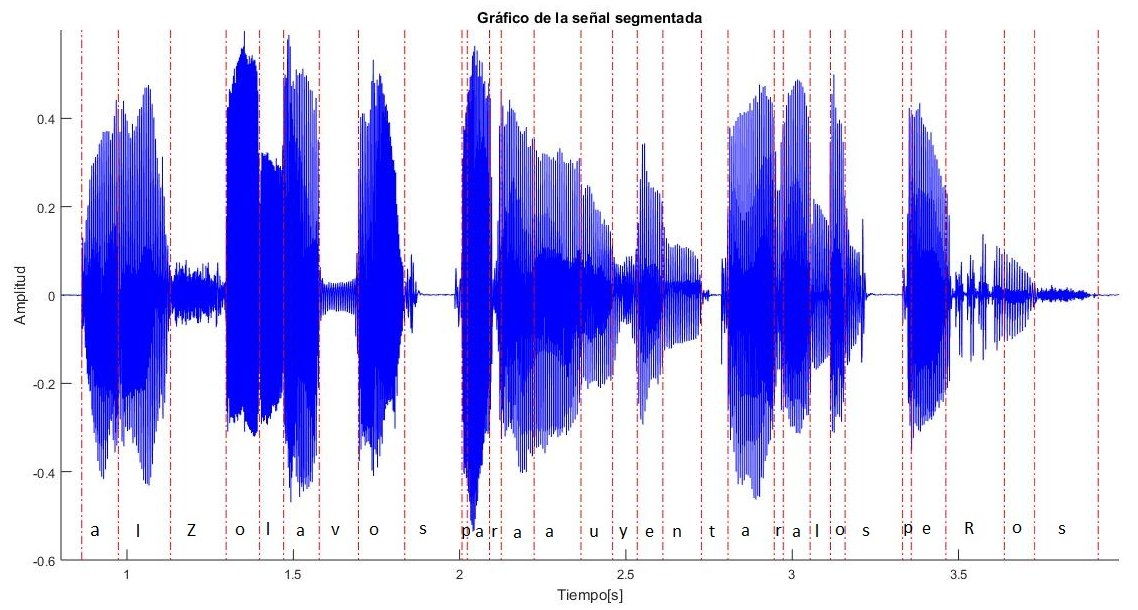
\includegraphics[scale=0.4]{Ejercicio_1.jpg}}


\subsection{Ejercicio 2}
	

\textit{Con la segmentación realizada en el ejercicio 1 de la señal} \texttt{hh2.wav}\emph{, encuentre los coeficientes
de Fourier de un período del segmento de señal correspondiente a un fono [a]. Repetir el cálculo
para varios períodos de la vocal.}\\

	A continuación se presenta el gráfico del fono [a] seleccionado, que corresponde a la última [a] de la palabra \emph{ahuyentar}. En ella también se presentan los periodos seleccionados para el cálculo de coeficientes.

	\begin{figure}
		\centering
		\scalebox{0.6}{% GNUPLOT: LaTeX picture with Postscript
\begingroup
  \makeatletter
  \providecommand\color[2][]{%
    \GenericError{(gnuplot) \space\space\space\@spaces}{%
      Package color not loaded in conjunction with
      terminal option `colourtext'%
    }{See the gnuplot documentation for explanation.%
    }{Either use 'blacktext' in gnuplot or load the package
      color.sty in LaTeX.}%
    \renewcommand\color[2][]{}%
  }%
  \providecommand\includegraphics[2][]{%
    \GenericError{(gnuplot) \space\space\space\@spaces}{%
      Package graphicx or graphics not loaded%
    }{See the gnuplot documentation for explanation.%
    }{The gnuplot epslatex terminal needs graphicx.sty or graphics.sty.}%
    \renewcommand\includegraphics[2][]{}%
  }%
  \providecommand\rotatebox[2]{#2}%
  \@ifundefined{ifGPcolor}{%
    \newif\ifGPcolor
    \GPcolorfalse
  }{}%
  \@ifundefined{ifGPblacktext}{%
    \newif\ifGPblacktext
    \GPblacktexttrue
  }{}%
  % define a \g@addto@macro without @ in the name:
  \let\gplgaddtomacro\g@addto@macro
  % define empty templates for all commands taking text:
  \gdef\gplbacktext{}%
  \gdef\gplfronttext{}%
  \makeatother
  \ifGPblacktext
    % no textcolor at all
    \def\colorrgb#1{}%
    \def\colorgray#1{}%
  \else
    % gray or color?
    \ifGPcolor
      \def\colorrgb#1{\color[rgb]{#1}}%
      \def\colorgray#1{\color[gray]{#1}}%
      \expandafter\def\csname LTw\endcsname{\color{white}}%
      \expandafter\def\csname LTb\endcsname{\color{black}}%
      \expandafter\def\csname LTa\endcsname{\color{black}}%
      \expandafter\def\csname LT0\endcsname{\color[rgb]{1,0,0}}%
      \expandafter\def\csname LT1\endcsname{\color[rgb]{0,1,0}}%
      \expandafter\def\csname LT2\endcsname{\color[rgb]{0,0,1}}%
      \expandafter\def\csname LT3\endcsname{\color[rgb]{1,0,1}}%
      \expandafter\def\csname LT4\endcsname{\color[rgb]{0,1,1}}%
      \expandafter\def\csname LT5\endcsname{\color[rgb]{1,1,0}}%
      \expandafter\def\csname LT6\endcsname{\color[rgb]{0,0,0}}%
      \expandafter\def\csname LT7\endcsname{\color[rgb]{1,0.3,0}}%
      \expandafter\def\csname LT8\endcsname{\color[rgb]{0.5,0.5,0.5}}%
    \else
      % gray
      \def\colorrgb#1{\color{black}}%
      \def\colorgray#1{\color[gray]{#1}}%
      \expandafter\def\csname LTw\endcsname{\color{white}}%
      \expandafter\def\csname LTb\endcsname{\color{black}}%
      \expandafter\def\csname LTa\endcsname{\color{black}}%
      \expandafter\def\csname LT0\endcsname{\color{black}}%
      \expandafter\def\csname LT1\endcsname{\color{black}}%
      \expandafter\def\csname LT2\endcsname{\color{black}}%
      \expandafter\def\csname LT3\endcsname{\color{black}}%
      \expandafter\def\csname LT4\endcsname{\color{black}}%
      \expandafter\def\csname LT5\endcsname{\color{black}}%
      \expandafter\def\csname LT6\endcsname{\color{black}}%
      \expandafter\def\csname LT7\endcsname{\color{black}}%
      \expandafter\def\csname LT8\endcsname{\color{black}}%
    \fi
  \fi
  \setlength{\unitlength}{0.0500bp}%
  \begin{picture}(11520.00,8640.00)%
    \gplgaddtomacro\gplbacktext{%
      \colorrgb{0.00,0.00,0.00}%
      \put(660,400){\makebox(0,0)[r]{\strut{}-0.8}}%
      \colorrgb{0.00,0.00,0.00}%
      \put(660,1355){\makebox(0,0)[r]{\strut{}-0.6}}%
      \colorrgb{0.00,0.00,0.00}%
      \put(660,2310){\makebox(0,0)[r]{\strut{}-0.4}}%
      \colorrgb{0.00,0.00,0.00}%
      \put(660,3265){\makebox(0,0)[r]{\strut{}-0.2}}%
      \colorrgb{0.00,0.00,0.00}%
      \put(660,4220){\makebox(0,0)[r]{\strut{}0}}%
      \colorrgb{0.00,0.00,0.00}%
      \put(660,5174){\makebox(0,0)[r]{\strut{}0.2}}%
      \colorrgb{0.00,0.00,0.00}%
      \put(660,6129){\makebox(0,0)[r]{\strut{}0.4}}%
      \colorrgb{0.00,0.00,0.00}%
      \put(660,7084){\makebox(0,0)[r]{\strut{}0.6}}%
      \colorrgb{0.00,0.00,0.00}%
      \put(660,8039){\makebox(0,0)[r]{\strut{}0.8}}%
      \colorrgb{0.00,0.00,0.00}%
      \put(976,200){\makebox(0,0){\strut{}2.8}}%
      \colorrgb{0.00,0.00,0.00}%
      \put(2281,200){\makebox(0,0){\strut{}2.82}}%
      \colorrgb{0.00,0.00,0.00}%
      \put(3587,200){\makebox(0,0){\strut{}2.84}}%
      \colorrgb{0.00,0.00,0.00}%
      \put(4892,200){\makebox(0,0){\strut{}2.86}}%
      \colorrgb{0.00,0.00,0.00}%
      \put(6198,200){\makebox(0,0){\strut{}2.88}}%
      \colorrgb{0.00,0.00,0.00}%
      \put(7504,200){\makebox(0,0){\strut{}2.9}}%
      \colorrgb{0.00,0.00,0.00}%
      \put(8809,200){\makebox(0,0){\strut{}2.92}}%
      \colorrgb{0.00,0.00,0.00}%
      \put(10115,200){\makebox(0,0){\strut{}2.94}}%
      \csname LTb\endcsname%
      \put(5969,8339){\makebox(0,0){\strut{}Gráfico del fono "a" (ahuyentar) con los periodos utilizados}}%
    }%
    \gplgaddtomacro\gplfronttext{%
      \colorrgb{0.00,0.00,0.00}%
      \put(2763,1563){\makebox(0,0)[r]{\strut{}Fono "a"}}%
      \colorrgb{0.00,0.00,0.00}%
      \put(2763,1363){\makebox(0,0)[r]{\strut{}Periodo 1}}%
      \colorrgb{0.00,0.00,0.00}%
      \put(2763,1163){\makebox(0,0)[r]{\strut{}Periodo 2}}%
      \colorrgb{0.00,0.00,0.00}%
      \put(2763,963){\makebox(0,0)[r]{\strut{}Periodo 3}}%
      \colorrgb{0.00,0.00,0.00}%
      \put(2763,763){\makebox(0,0)[r]{\strut{}Periodo 4}}%
      \colorrgb{0.00,0.00,0.00}%
      \put(2763,563){\makebox(0,0)[r]{\strut{}Periodo 5}}%
    }%
    \gplbacktext
    \put(0,0){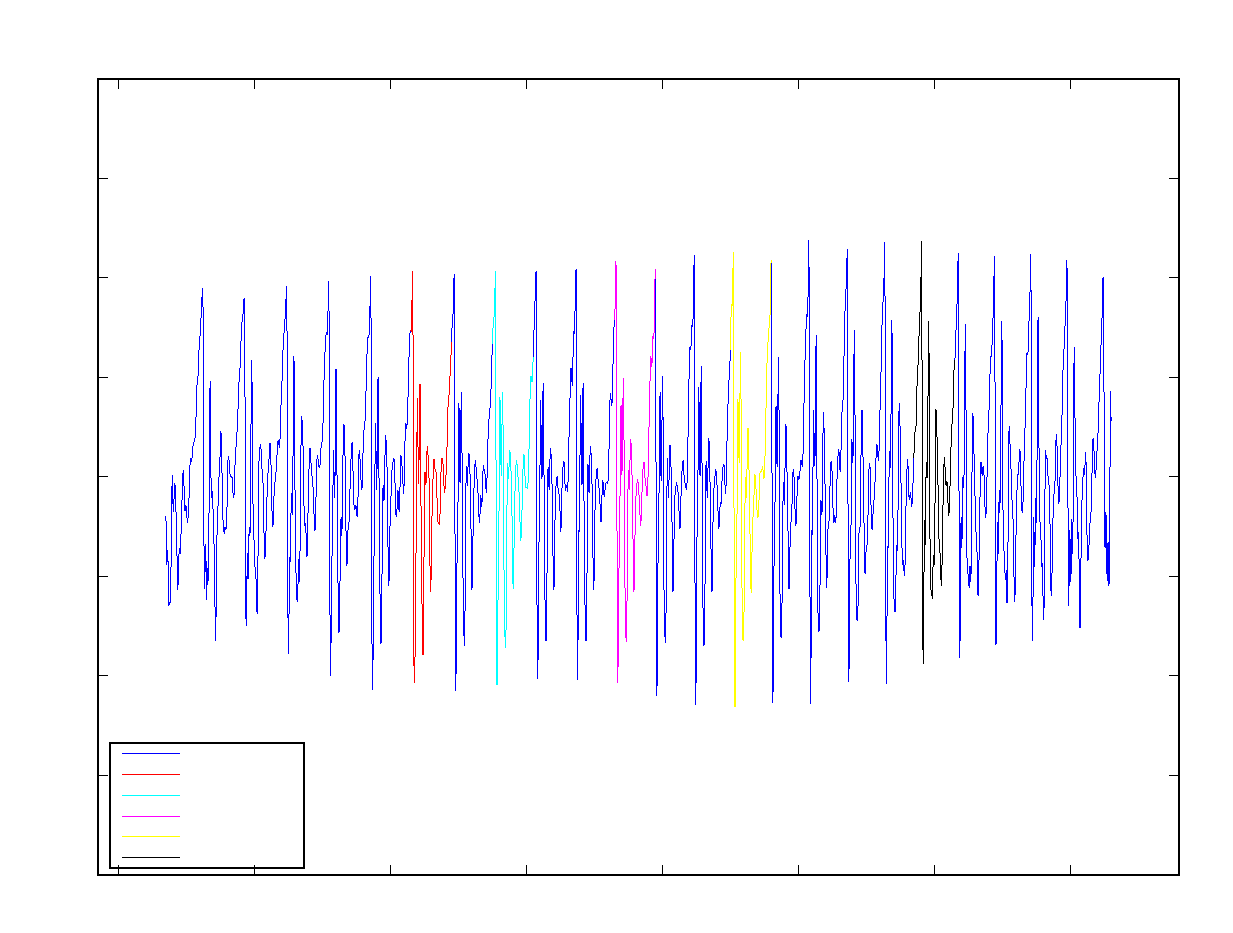
\includegraphics{./graf_fono_a}}%
    \gplfronttext
  \end{picture}%
\endgroup
}
	\end{figure}

	Con los periodos seleccionados previamente, se obtuvieron los coeficientes de Fourier, representados en el siguiente gráfico

	
	\begin{figure}
		\centering
		\scalebox{0.6}{% GNUPLOT: LaTeX picture with Postscript
\begingroup
  \makeatletter
  \providecommand\color[2][]{%
    \GenericError{(gnuplot) \space\space\space\@spaces}{%
      Package color not loaded in conjunction with
      terminal option `colourtext'%
    }{See the gnuplot documentation for explanation.%
    }{Either use 'blacktext' in gnuplot or load the package
      color.sty in LaTeX.}%
    \renewcommand\color[2][]{}%
  }%
  \providecommand\includegraphics[2][]{%
    \GenericError{(gnuplot) \space\space\space\@spaces}{%
      Package graphicx or graphics not loaded%
    }{See the gnuplot documentation for explanation.%
    }{The gnuplot epslatex terminal needs graphicx.sty or graphics.sty.}%
    \renewcommand\includegraphics[2][]{}%
  }%
  \providecommand\rotatebox[2]{#2}%
  \@ifundefined{ifGPcolor}{%
    \newif\ifGPcolor
    \GPcolorfalse
  }{}%
  \@ifundefined{ifGPblacktext}{%
    \newif\ifGPblacktext
    \GPblacktexttrue
  }{}%
  % define a \g@addto@macro without @ in the name:
  \let\gplgaddtomacro\g@addto@macro
  % define empty templates for all commands taking text:
  \gdef\gplbacktext{}%
  \gdef\gplfronttext{}%
  \makeatother
  \ifGPblacktext
    % no textcolor at all
    \def\colorrgb#1{}%
    \def\colorgray#1{}%
  \else
    % gray or color?
    \ifGPcolor
      \def\colorrgb#1{\color[rgb]{#1}}%
      \def\colorgray#1{\color[gray]{#1}}%
      \expandafter\def\csname LTw\endcsname{\color{white}}%
      \expandafter\def\csname LTb\endcsname{\color{black}}%
      \expandafter\def\csname LTa\endcsname{\color{black}}%
      \expandafter\def\csname LT0\endcsname{\color[rgb]{1,0,0}}%
      \expandafter\def\csname LT1\endcsname{\color[rgb]{0,1,0}}%
      \expandafter\def\csname LT2\endcsname{\color[rgb]{0,0,1}}%
      \expandafter\def\csname LT3\endcsname{\color[rgb]{1,0,1}}%
      \expandafter\def\csname LT4\endcsname{\color[rgb]{0,1,1}}%
      \expandafter\def\csname LT5\endcsname{\color[rgb]{1,1,0}}%
      \expandafter\def\csname LT6\endcsname{\color[rgb]{0,0,0}}%
      \expandafter\def\csname LT7\endcsname{\color[rgb]{1,0.3,0}}%
      \expandafter\def\csname LT8\endcsname{\color[rgb]{0.5,0.5,0.5}}%
    \else
      % gray
      \def\colorrgb#1{\color{black}}%
      \def\colorgray#1{\color[gray]{#1}}%
      \expandafter\def\csname LTw\endcsname{\color{white}}%
      \expandafter\def\csname LTb\endcsname{\color{black}}%
      \expandafter\def\csname LTa\endcsname{\color{black}}%
      \expandafter\def\csname LT0\endcsname{\color{black}}%
      \expandafter\def\csname LT1\endcsname{\color{black}}%
      \expandafter\def\csname LT2\endcsname{\color{black}}%
      \expandafter\def\csname LT3\endcsname{\color{black}}%
      \expandafter\def\csname LT4\endcsname{\color{black}}%
      \expandafter\def\csname LT5\endcsname{\color{black}}%
      \expandafter\def\csname LT6\endcsname{\color{black}}%
      \expandafter\def\csname LT7\endcsname{\color{black}}%
      \expandafter\def\csname LT8\endcsname{\color{black}}%
    \fi
  \fi
  \setlength{\unitlength}{0.0500bp}%
  \begin{picture}(11520.00,8640.00)%
    \gplgaddtomacro\gplbacktext{%
      \colorrgb{0.00,0.00,0.00}%
      \put(500,640){\makebox(0,0)[r]{\strut{}0}}%
      \colorrgb{0.00,0.00,0.00}%
      \put(500,1565){\makebox(0,0)[r]{\strut{}1}}%
      \colorrgb{0.00,0.00,0.00}%
      \put(500,2490){\makebox(0,0)[r]{\strut{}2}}%
      \colorrgb{0.00,0.00,0.00}%
      \put(500,3415){\makebox(0,0)[r]{\strut{}3}}%
      \colorrgb{0.00,0.00,0.00}%
      \put(500,4340){\makebox(0,0)[r]{\strut{}4}}%
      \colorrgb{0.00,0.00,0.00}%
      \put(500,5264){\makebox(0,0)[r]{\strut{}5}}%
      \colorrgb{0.00,0.00,0.00}%
      \put(500,6189){\makebox(0,0)[r]{\strut{}6}}%
      \colorrgb{0.00,0.00,0.00}%
      \put(500,7114){\makebox(0,0)[r]{\strut{}7}}%
      \colorrgb{0.00,0.00,0.00}%
      \put(500,8039){\makebox(0,0)[r]{\strut{}8}}%
      \colorrgb{0.00,0.00,0.00}%
      \put(620,440){\makebox(0,0){\strut{}0}}%
      \colorrgb{0.00,0.00,0.00}%
      \put(1937,440){\makebox(0,0){\strut{}500}}%
      \colorrgb{0.00,0.00,0.00}%
      \put(3255,440){\makebox(0,0){\strut{}1000}}%
      \colorrgb{0.00,0.00,0.00}%
      \put(4572,440){\makebox(0,0){\strut{}1500}}%
      \colorrgb{0.00,0.00,0.00}%
      \put(5890,440){\makebox(0,0){\strut{}2000}}%
      \colorrgb{0.00,0.00,0.00}%
      \put(7207,440){\makebox(0,0){\strut{}2500}}%
      \colorrgb{0.00,0.00,0.00}%
      \put(8524,440){\makebox(0,0){\strut{}3000}}%
      \colorrgb{0.00,0.00,0.00}%
      \put(9842,440){\makebox(0,0){\strut{}3500}}%
      \colorrgb{0.00,0.00,0.00}%
      \put(11159,440){\makebox(0,0){\strut{}4000}}%
      \colorrgb{0.00,0.00,0.00}%
      \put(160,4339){\rotatebox{90}{\makebox(0,0){\strut{}|X|}}}%
      \colorrgb{0.00,0.00,0.00}%
      \put(5889,140){\makebox(0,0){\strut{}Frecuencia [Hz]}}%
      \csname LTb\endcsname%
      \put(5889,8339){\makebox(0,0){\strut{}Respuesta en frecuencia de los periodos seleccionados del fono "a" (ahuyentar)}}%
    }%
    \gplgaddtomacro\gplfronttext{%
      \colorrgb{0.00,0.00,0.00}%
      \put(11039,7876){\makebox(0,0)[r]{\strut{}Periodo 1}}%
      \colorrgb{0.00,0.00,0.00}%
      \put(11039,7676){\makebox(0,0)[r]{\strut{}Periodo 2}}%
      \colorrgb{0.00,0.00,0.00}%
      \put(11039,7476){\makebox(0,0)[r]{\strut{}Periodo 3}}%
      \colorrgb{0.00,0.00,0.00}%
      \put(11039,7276){\makebox(0,0)[r]{\strut{}Periodo 4}}%
      \colorrgb{0.00,0.00,0.00}%
      \put(11039,7076){\makebox(0,0)[r]{\strut{}Periodo 5}}%
    }%
    \gplbacktext
    \put(0,0){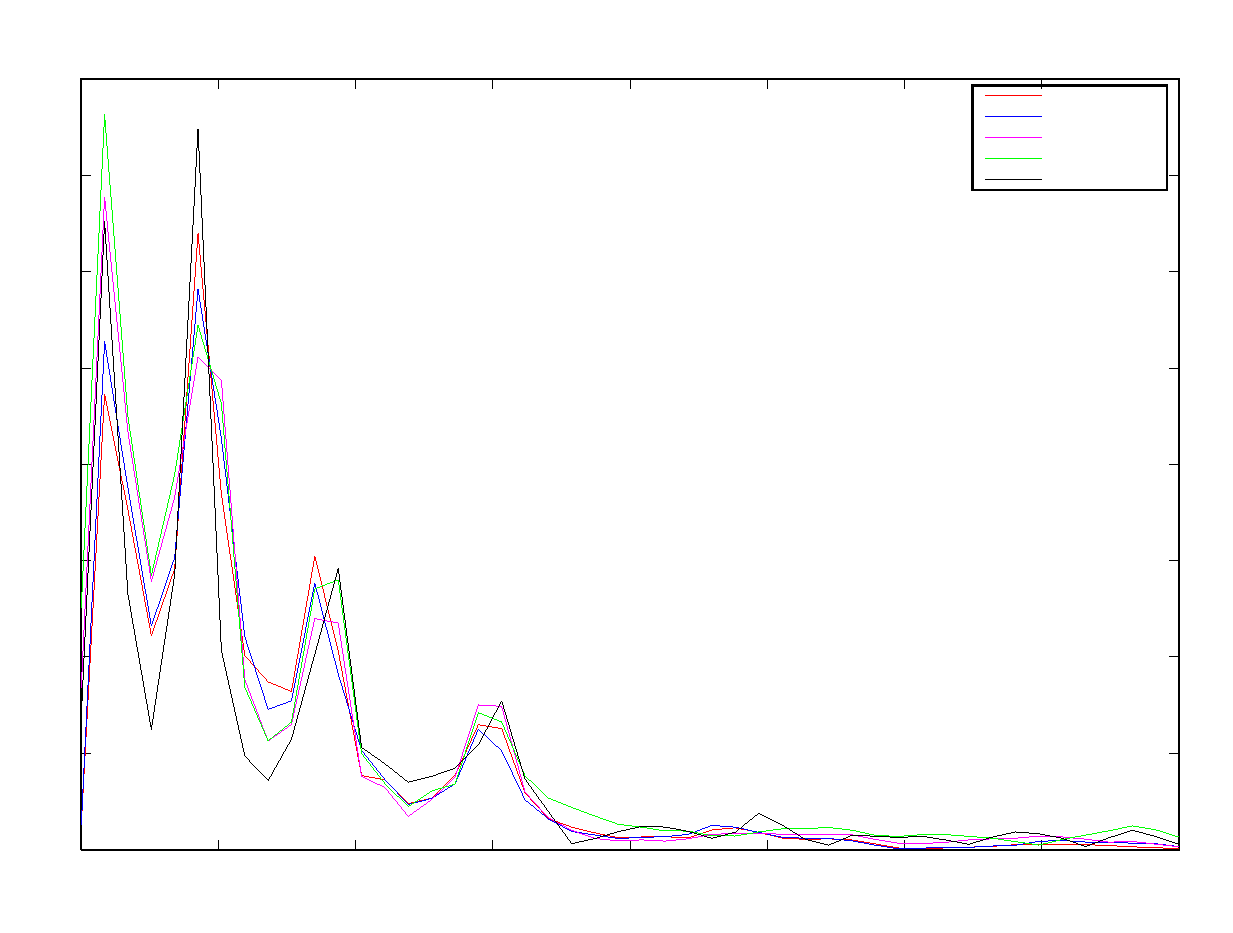
\includegraphics{./graf_coef}}%
    \gplfronttext
  \end{picture}%
\endgroup
}
	\end{figure}


\subsection{Ejercicio 3}
	

\textit{Reconstruya la señal temporal a partir de los coeficientes calculados. Escuche y compare las
distintas reconstrucciones correspondientes a coeficientes de Fourier tomados de distintos
períodos. Compárelas también con la señal original. ¿Qué observación se puede hacer sobre la
periodicidad de los fonemas vocálicos?}



\subsection{Ejercicio 4}
	


\textit{Grabe la misma frase del ejercicio 1. Mencionar las diferencias entre ambas señales.}



\subsection{Ejercicio 5}
	


\textit{Grafique los espectrogramas de banda angosta de los segmentos de señal correspondientes a
tres vocales presentes en la señal} \texttt{hh2.wav}\textit{. Compare y analice las diferencias.}



\subsection{Ejercicio 6}
	


\textit{Genere diez ciclos del tren de pulsos glóticos según los modelos de Rosenberg. Tomar una
frecuencia F0 = 200 Hz, y fases de apertura y cierre de 40\% y 16\%, respectivamente, de la
duración de un pulso. Considerar una amplitud máxima de 1. A los efectos de la simulación,
considerar una frecuencia de muestreo de 16 kHz. Estimar su espectro de amplitud y explicar su
contenido.}



\subsection{Ejercicio 7}
	
	\begin{equation}
		H_n(z)=\frac{1}{(1-p_n \cdot z^{-1})(1-p_n^* \cdot z^{-1})}
		\label{ec:transferencia}
	\end{equation}

	\begin{equation}
		p_n=e^{\frac{-2 \cdot \pi \cdot B}{F_s}} \cdot e^{j \cdot \frac{2 \cdot \pi \cdot F_n}{F_s}}
		\label{ec:polos}
	\end{equation}


\textit{Utilizando las ec. \ref{ec:transferencia} y \ref{ec:polos}, generar un modelo de tracto vocal para cada uno de los siguientes
conjuntos de valores de parámetros, que se corresponde con una vocal emitida por una locutora.}
\begin{table}[h!]
	\centering
	\begin{tabular}{*{9}{c}}
\toprule
	 	&$F_1$	&$B_1$	&$F_2$	&$B_2$	&$F_3$	&$B_3$	&$F_4$	&$B_4$	\\
\midrule
	a	&830	&110	&1400	&160	&2890	&210	&3930	&230	\\
	e	&500	&80	&2000	&156	&3130	&190	&4150	&220	\\
	i	&330	&70	&2765	&130	&3740	&178	&4366	&200	\\
	o	&546	&97	&934	&130	&2966	&185	&3930	&240	\\
	u	&382	&74	&740	&150	&2760	&210	&3380	&180	\\
\bottomrule
	\end{tabular}
\end{table}
\textit{Grafique diagrama de polos y ceros, y la respuesta en frecuencia del sistema para cada vocal, y
compare.}




\subsection{Ejercicio 8}
	


\emph{Utilizando los resultados de los dos último ejercicios, sintetice un segundo de las cinco vocales.
Escuche y grafique. Haga un análisis en frecuencia, y en tiempo-frecuencia.}



\subsection{Ejercicio 9}
	


\emph{Aplicando el método descripto en la introducción, estime el contorno de la frecuencia fundamental
de la voz en el archivo} \texttt{hh2.wav}\emph{. Grafique en forma sincrónica con la onda.}



\subsection{Ejercicio 10}
	


\emph{Con el resultado del ejercicio 9, aplique el método PSOLA para aumentar y disminuir un 10\%,
20\% y 30\% los valores de frecuencia en el contorno de F0 de la voz en el archivo} \texttt{hh2.wav}.



Hay que hacer algo automático, un porgrama que busque los máximos y eso. Hacer lo que dice ROdri.
No hacerlo si no se llega



Cuando veo que se me alarga y fue tantos periodso, los saco. No importa si sea alarga. Se agregan o se tiran periodos completos, nunca por partes.


\subsection{Ejercicio 11}
	


\emph{Repita el ejercicio 10 pero aplicando el método para ajustar la velocidad del habla.}



No tiene nada que ver con el 10. Hay que cambiar la velocidad. O sea lo que hizo rodri. Podría cambiar la frecuencia de muestreo.


Con humberto

Dejar la frecuencia como está y se agregan o se sacan periódos para aumentar o subir la velocidad.


\subsection{Ejercicio 12}
	


\emph{Repita el ejercicio 8, pero variando la frecuencia fundamental desde 200 Hz a 300 Hz en forma
lineal. Escuche la onda resultante, ¿cómo se percibe el cambio en la frecuencia fundamental?
Estime el F0 resultante y compárelo con el teórico.}



\subsection{Ejercicio 13}
	


\emph{Repita el ejercicio 12, pero variando la frecuencia fundamental desde 200 Hz a 100 Hz.}



\subsection{Ejercicio 14}
	


\emph{A la señal de vocales generada en el ejercicio 8 realícele un filtrado con el objetivo de eliminar su
frecuencia fundamental. Puede utilizar la herramienta fdatool para diseñar el filtro. Justifique el
filtro implementado. Grafique ambas señales, haga un análisis en frecuencia y compare.
¿Perceptualmente se percibe alguna diferencia? ¿Porqué?}



	
	\section{Código fuente}
%		

	\lstinputlisting{tp.m}



\end{document}
